\documentclass[simplex.tex]{subfiles}
% NO NEED TO INPUT PREAMBLES HERE
% packages are inherited; you can compile this on its own

\onlyinsubfile{
\title{NeuroData SIMPLEX Report: Subfile}
}

\begin{document}
\onlyinsubfile{
\maketitle
\thispagestyle{empty}

The following report documents the progress made by the labs of Randal~Burns and Joshua~T.~Vogelstein at Johns Hopkins University towards goals set by the DARPA SIMPLEX grant.

%%%% Table of Contents
\tableofcontents

%%%% Publications
\bibliographystyle{IEEEtran}
\begin{spacing}{0.5}
\section*{Publications, Presentations, and Talks}
%\vspace{-20pt}
\nocite{*}
{\footnotesize	\bibliography{simplex}}
\end{spacing}
%%%% End Publications
}

\subsection{Non-Parametric Shape Clustering}

We are developing non-parametric methods to cluster shapes. A shape
consists in the geometric information contained in an object, which
is scaling, translational, and rotational invariant. Our method consists
in applying a modified version of k-means algorithm which incorporates a
mathematical metric between shapes based on Procrustes alignment. This
can have several applications, and we are particularly interested in
using this technique to analyze similarities between neural synapses. As
an example, the figure~\ref{fig:nonparShape} illustrates the shape extraction and
alignment between two handwritten digits. Using the distance provided by
this method, we are able to cluster three classes of digits more
accurately than pure k-means method. 

\begin{figure}[h!]
\begin{cframed}
\centering
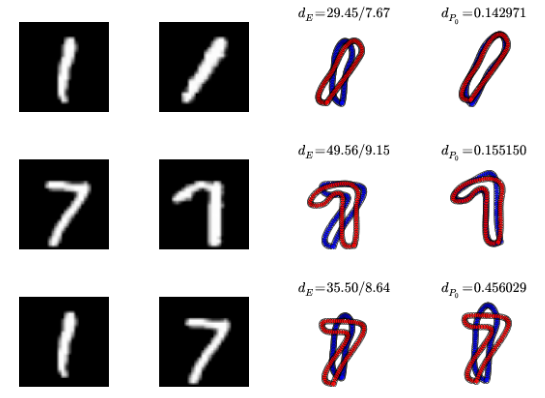
\includegraphics[width=0.75\textwidth]{../../figs/nonparShape.png}
\caption{
 Example: shape extraction and alignment between two handwritten digits.
}
\label{fig:nonparShape}
\end{cframed}
\end{figure}

\begin{figure}[h!]
\begin{cframed}
\centering
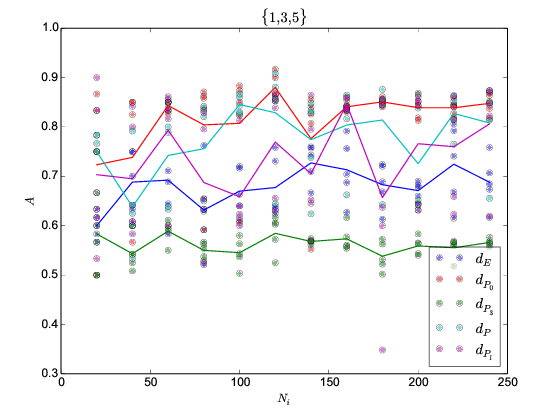
\includegraphics[width=0.75\textwidth]{../../figs/nonpar135.png}
\caption{
The graph shows the accuracy
(1 is the best possible) versus the number of elements in each class.
Our shape clustering methods (red and cyan lines) are more accurate than
k-means based on Euclidean distance (blue, magenta, and green lines). In
this example the accuracy is around 85\%, which is quite good for
unsupervised clustering on this dataset.
}
\label{fig:nonpar135}
\end{cframed}
\end{figure}

To test our algorithm we used the well-known MNIST handwritten digits
dataset. For each digit we extract landmark points, and align them
through Procrustes. This procedure defines a distance between any two
objects, and is illustrated in figure~\ref{fig:nonpar}~(a). Using this
distance we then cluster three classes of digits using a modified
K-means algorithm. 

The example shown in figure~\ref{fig:nonpar}~(b)
shows a pretty low error, around 10\%, for an unsupervised clustering
method.

\begin{figure}[h!]
\begin{cframed}
\centering

\begin{subfigure}[t]{0.45\textwidth}
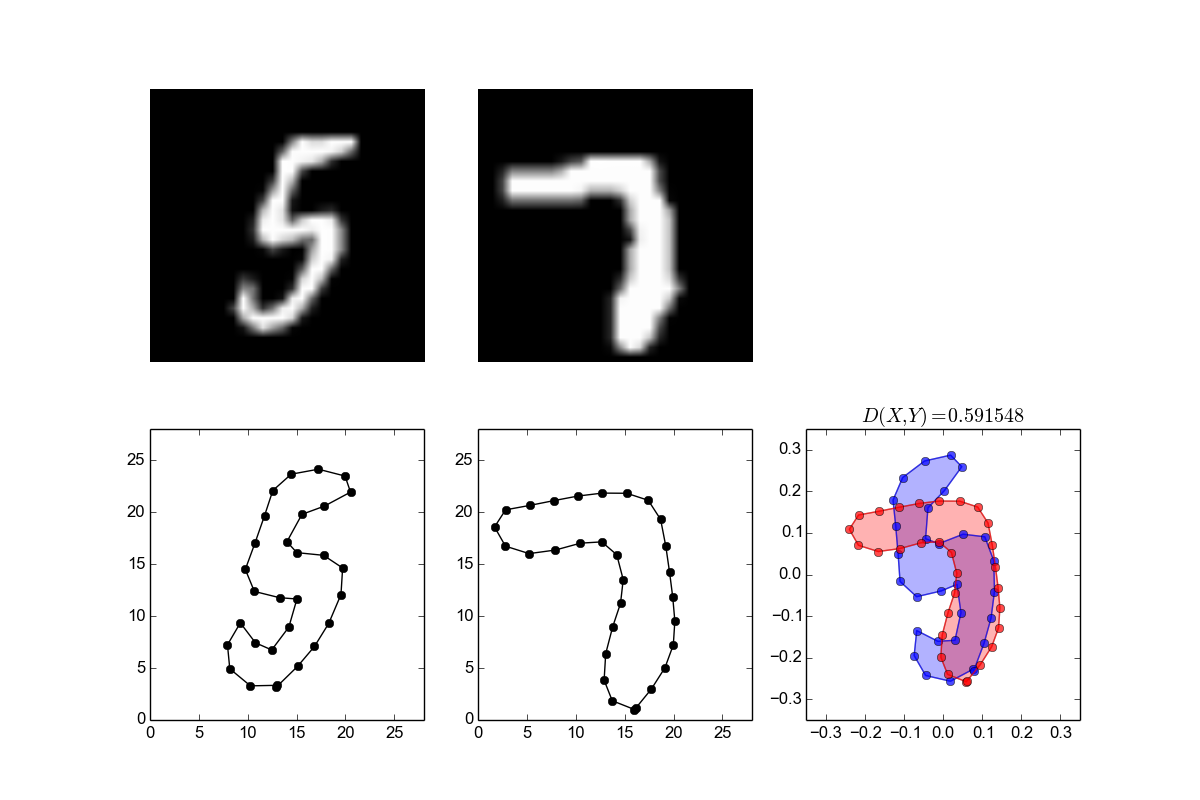
\includegraphics[width=\textwidth]{../../figs/nonpar57.png}
\label{fig:nonpar57}
\caption{
  MNIST digits with extracted landmarks and alignment.
  }
\end{subfigure}
\begin{subfigure}[t]{0.45\textwidth}
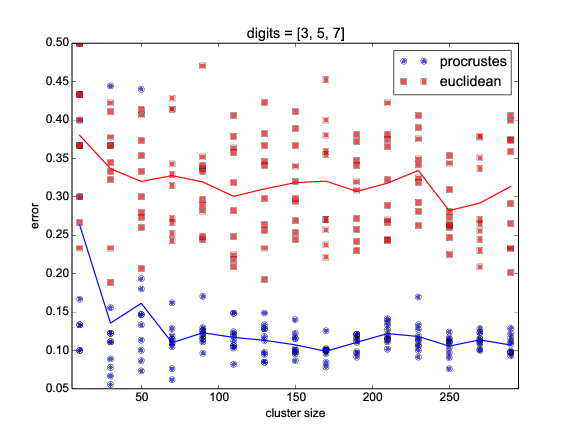
\includegraphics[width=\textwidth]{../../figs/nonPar357.png}
\label{fig:nonpar357}
\caption{
Classification error against the size of each
cluster --- the three classes have the same number of points --- is
shown in blue. The red line is standard
K-means with Euclidean distance for comparison.   }
\end{subfigure}
\caption{
  MNIST data and classification error results.
}
\label{fig:nonpar}
\end{cframed}
\end{figure}

\end{document}
